\documentclass[11pt,letterpaper]{article}
\usepackage{fullpage}

\usepackage[english]{babel}
\usepackage[utf8]{inputenc}
\usepackage{amsmath}
\usepackage{graphicx}
\usepackage[hidelinks]{hyperref}
\usepackage{float}
\usepackage{amsfonts}
\usepackage{algorithm,algpseudocode}
\usepackage{pdfpages}
             
\graphicspath{{../results}}

\begin{document} 

\title{Experiment 2}
\maketitle

\section*{Simulation Details}

Considered $K = 3$, $T = 1001$, $N = 500$. Report statistics at $t = 1000$ \\
\textbf{The Bandit priors that were considered}:
\begin{itemize}
\item Uniform: Draw the mean rewards for the arms from [0.25, 0.75]
\item ``HeavyTail": We took the mean rewards to be randomly drawn from Beta($\alpha=0.6,\beta=0.6$). With this distribution it was likely to have arms that were at the extremes (close to 1 and close to 0) but also some of the arms with intermediate value means.
\item Needle-in-haystack
\begin{enumerate}
\item High - 2 arms with mean 0.50, 1 arm with mean 0.70 (+ 0.20)
\end{enumerate}
\end{itemize}
\textbf{Algorithms considered}:
\begin{enumerate}
\item ThompsonSampling with priors of $Beta(1, 1)$ for every arm.
\item DynamicGreedy with priors of $Beta(1, 1)$ for every arm
\item Bayesian Dynamic $\epsilon$-greedy with priors of $Beta(1, 1)$ for every arm and $\epsilon=0.05$
\end{enumerate}
\textbf{Agent Algorithms considered}:
\begin{enumerate}
\item HardMax
\item HardMaxWithRandom
\item SoftMax ($\alpha = 10$)
\end{enumerate}
\textbf{Memory Sizes}
\begin{enumerate}
\item 100
\end{enumerate}
\pagebreak
\textbf{Simulation Procedure}
\begin{algorithm}
\begin{algorithmic}[1]
\For{Each prior $p$}
\State Generate true distribution from $p$ (except for needle-in-haystack, just use $p$ itself)
\State Generate $T \times K$ realizations for the arms 
	\For{Each agent algorithm $agent alg$}
		\For{Each principal algorithm pair $principalalg1$, $principalalg2$}
			\For{$N$ simulations}
				
				\State Give the agents 5 observations from each principal
				\State Give principal 2 200 free observations (the agents also get these observations)
				\State Run simulation for T periods
			\EndFor
		\EndFor
	\EndFor
\EndFor
\end{algorithmic}
\end{algorithm}

\section*{Results}
All results are reported for memory size = 100. \\
\vspace{0.25cm}

The rows represent Principal 1 and the columns represent Principal 2. Thus, the cell (1, 2) represents principal 1 playing Thompson Sampling and principal 2 playing DynamicEpsilonGreedy. In this experiment remember that principal 2 gets 200 free observations.  \\
\vspace{0.1cm}

Within each cell, the following data are presented: \\

\begin{enumerate}
\item The first row displays the sample mean market share for principal 1 as well as a 95\% confidence band of the mean.

\item The second row displays the sample variance of the market share and in parentheses are 95 \% confidence bands for the variance.

\item The third row displays the \% of simulations that resulted in ``extreme" market shares. Extreme market shares are defined as being simulations were one of the principals (either principal 1 or 2) ended up with 90\% or more of the market.
\end{enumerate}
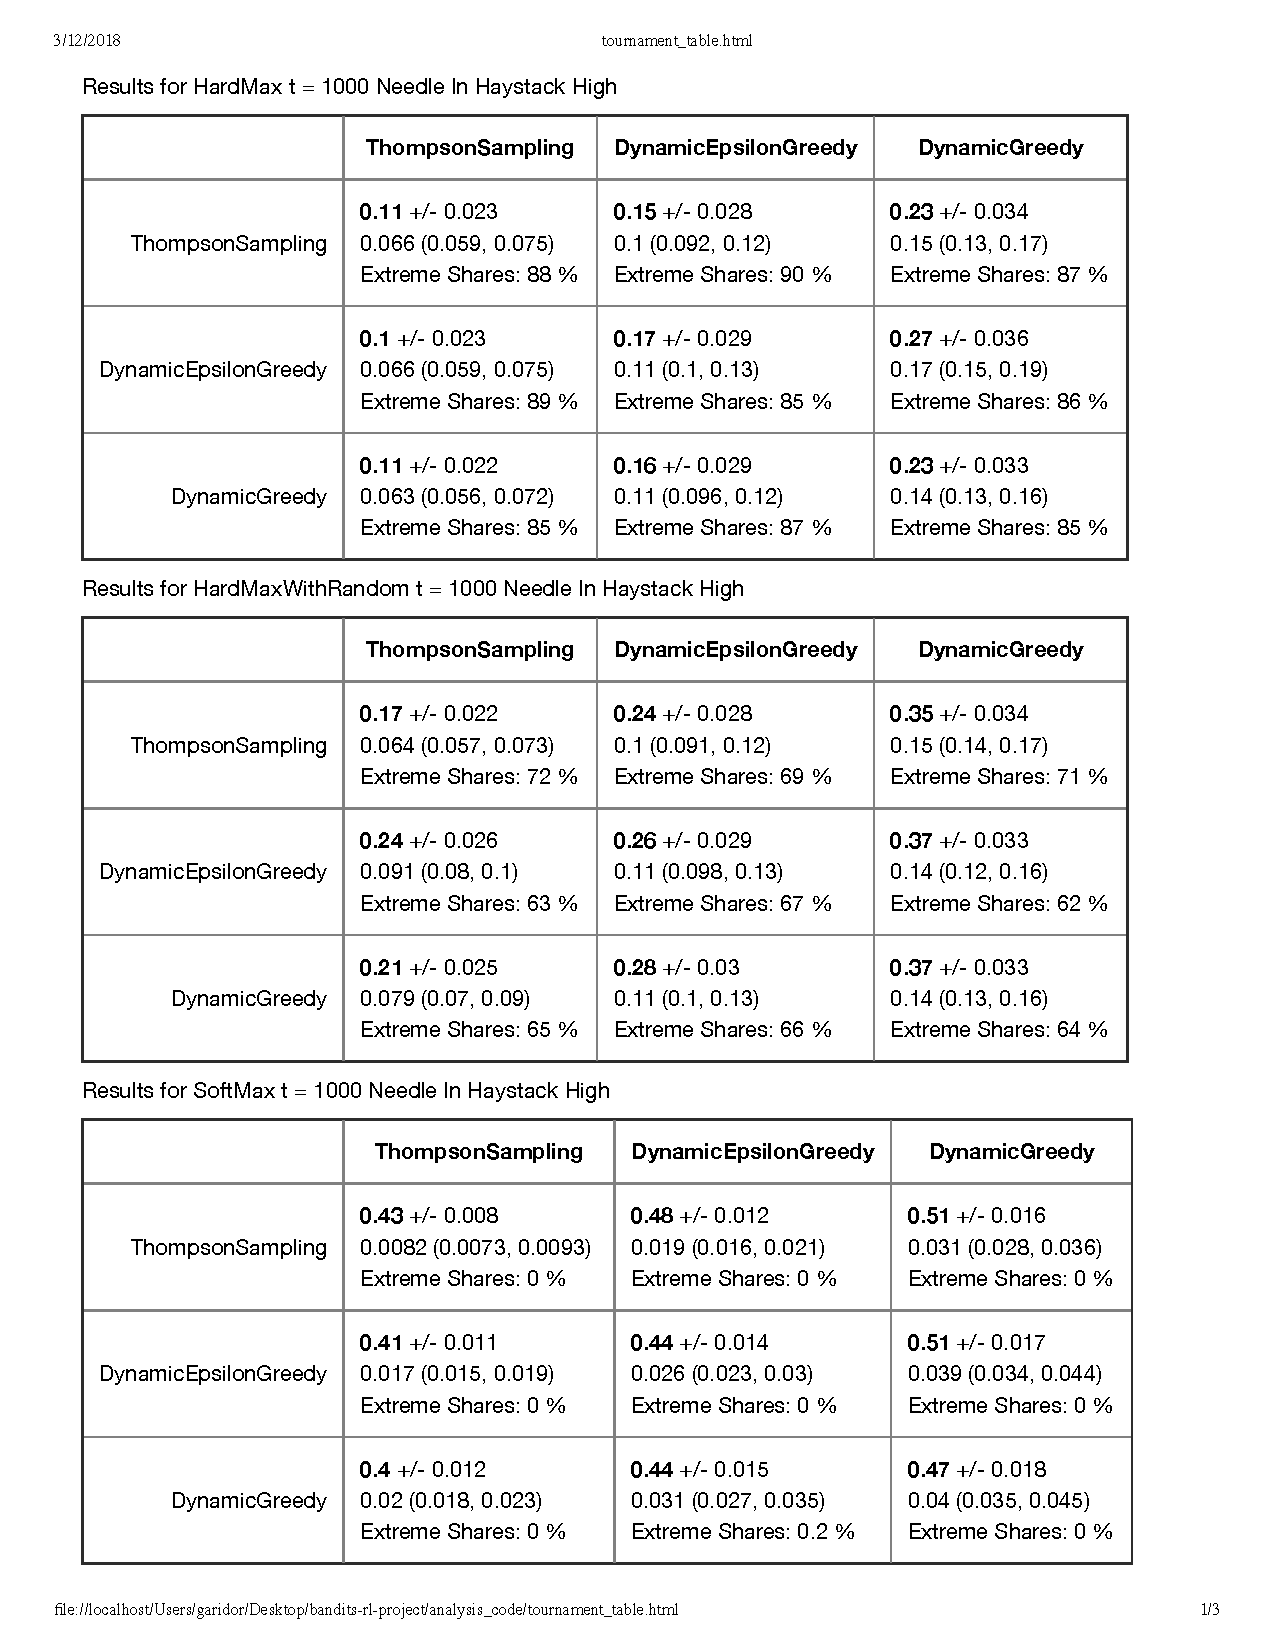
\includepdf[pages={-}]{tournament_table}

Comments: The story I seem to get from this is (roughly) that the worse the algorithm that the incumbent plays is, the better the entrant will do. Thus, the incumbent should want to play a better algorithm. However, in order for the entrant to do as well as possible, the entrant should in fact play a worse algorithm! If you think of it from the incumbent point of view, the incumbent is in the market first and so wants to learn as much as possible before the entrant comes in (thus does better with a better algorithm since it should have learned more by the time the entrant enters).  From the entrant point of view, since the incumbent has already learned something in order to have any chance to compete you do better by purely exploiting than by engaging in potentially suboptimal exploration. Two follow-up questions: Will this result hold if we run the simulations for more periods? What will happen to this result if we increase memory size? Another question is whether or not the effect is driven by the better information the incumbent has or the effect of reputation.
\vspace{0.5cm}

This motivates the following experiment which has an identical setup as before (principal 2 gets to be in the game for 200 periods before principal 1), however after the 200 rounds we are going to erase the memory of the agents. Thus, when principal 1 enters the market the incumbent (principal 2) does not have an advantage in terms of reputation, but only in terms of the information s/he possesses. The results don't change much qualitatively from the case we first considered.
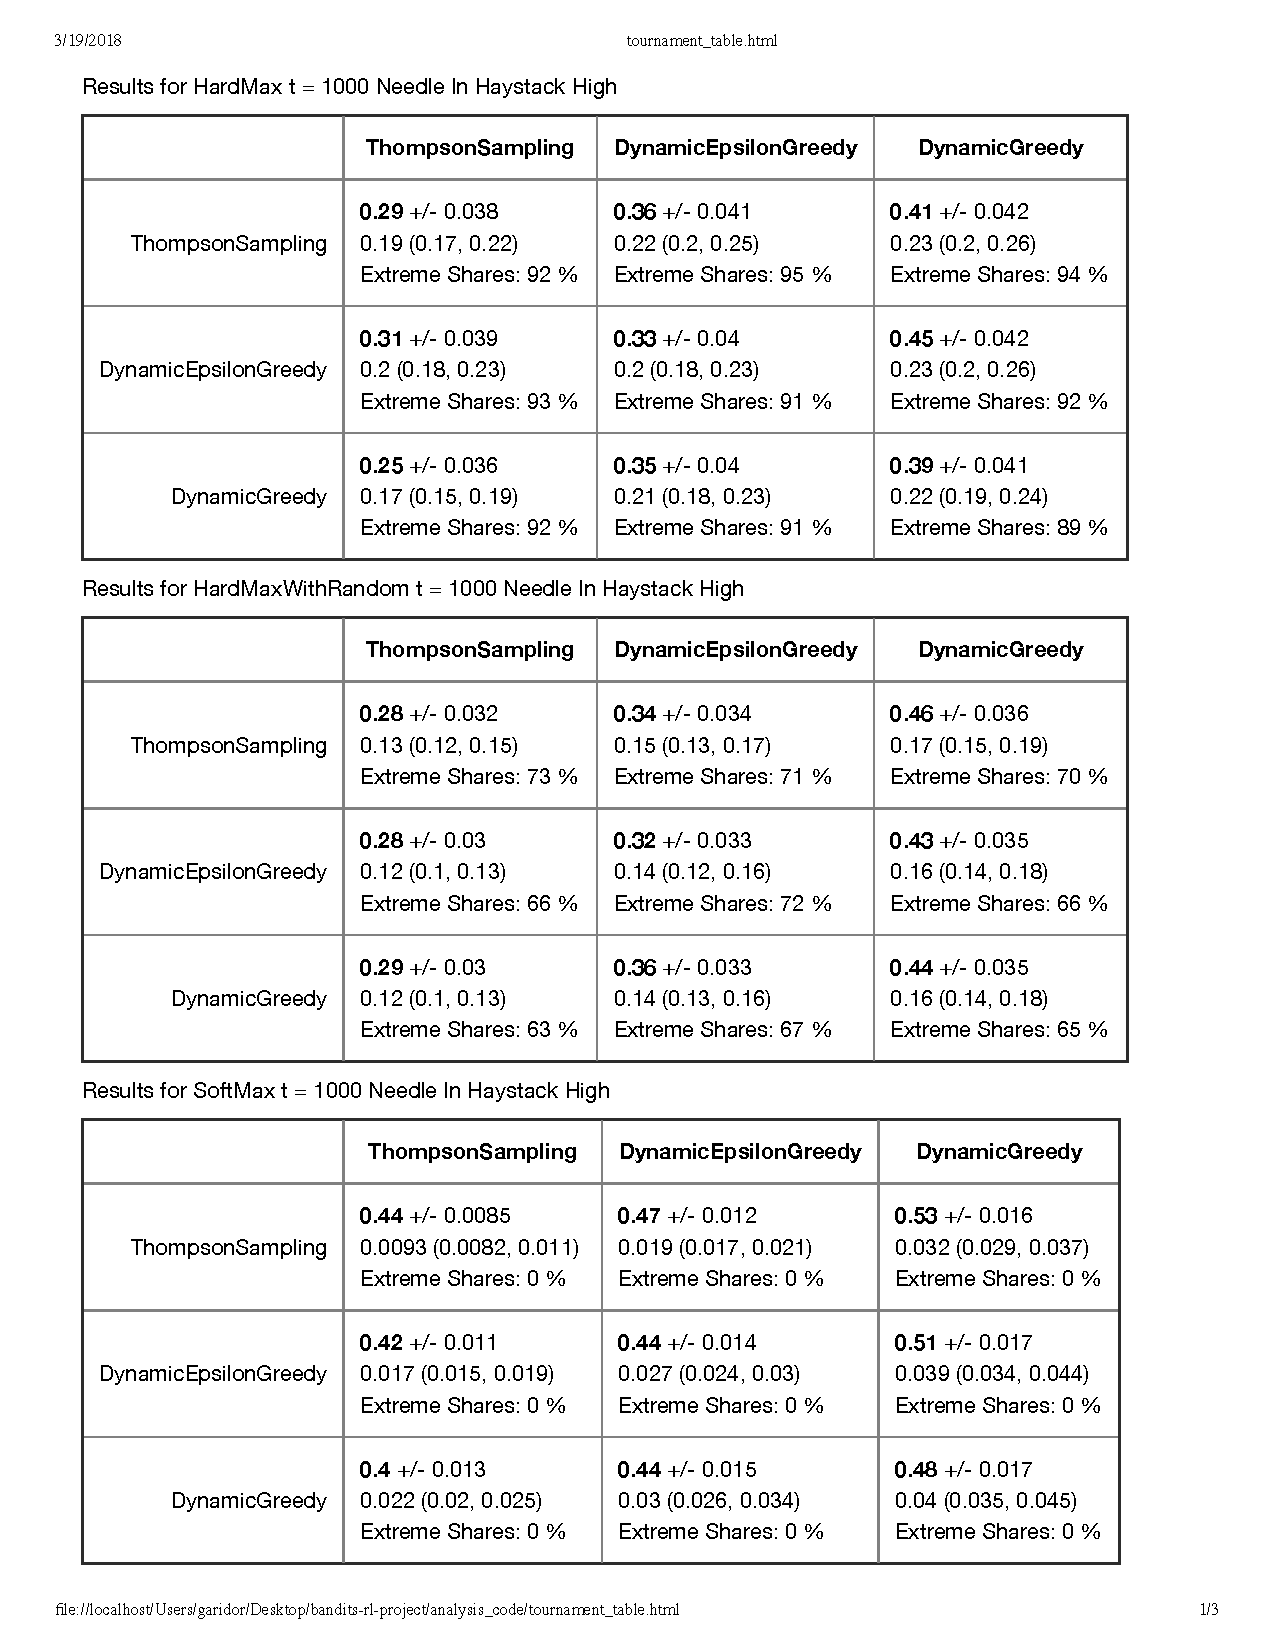
\includepdf[pages={-}]{no_reputation_tournament_table}

Another check of the robustness of the results: The memory size is increased to 250 so that when principal 1 enters the market the entire history of the incumbent is contained in the information set of the incumbent.
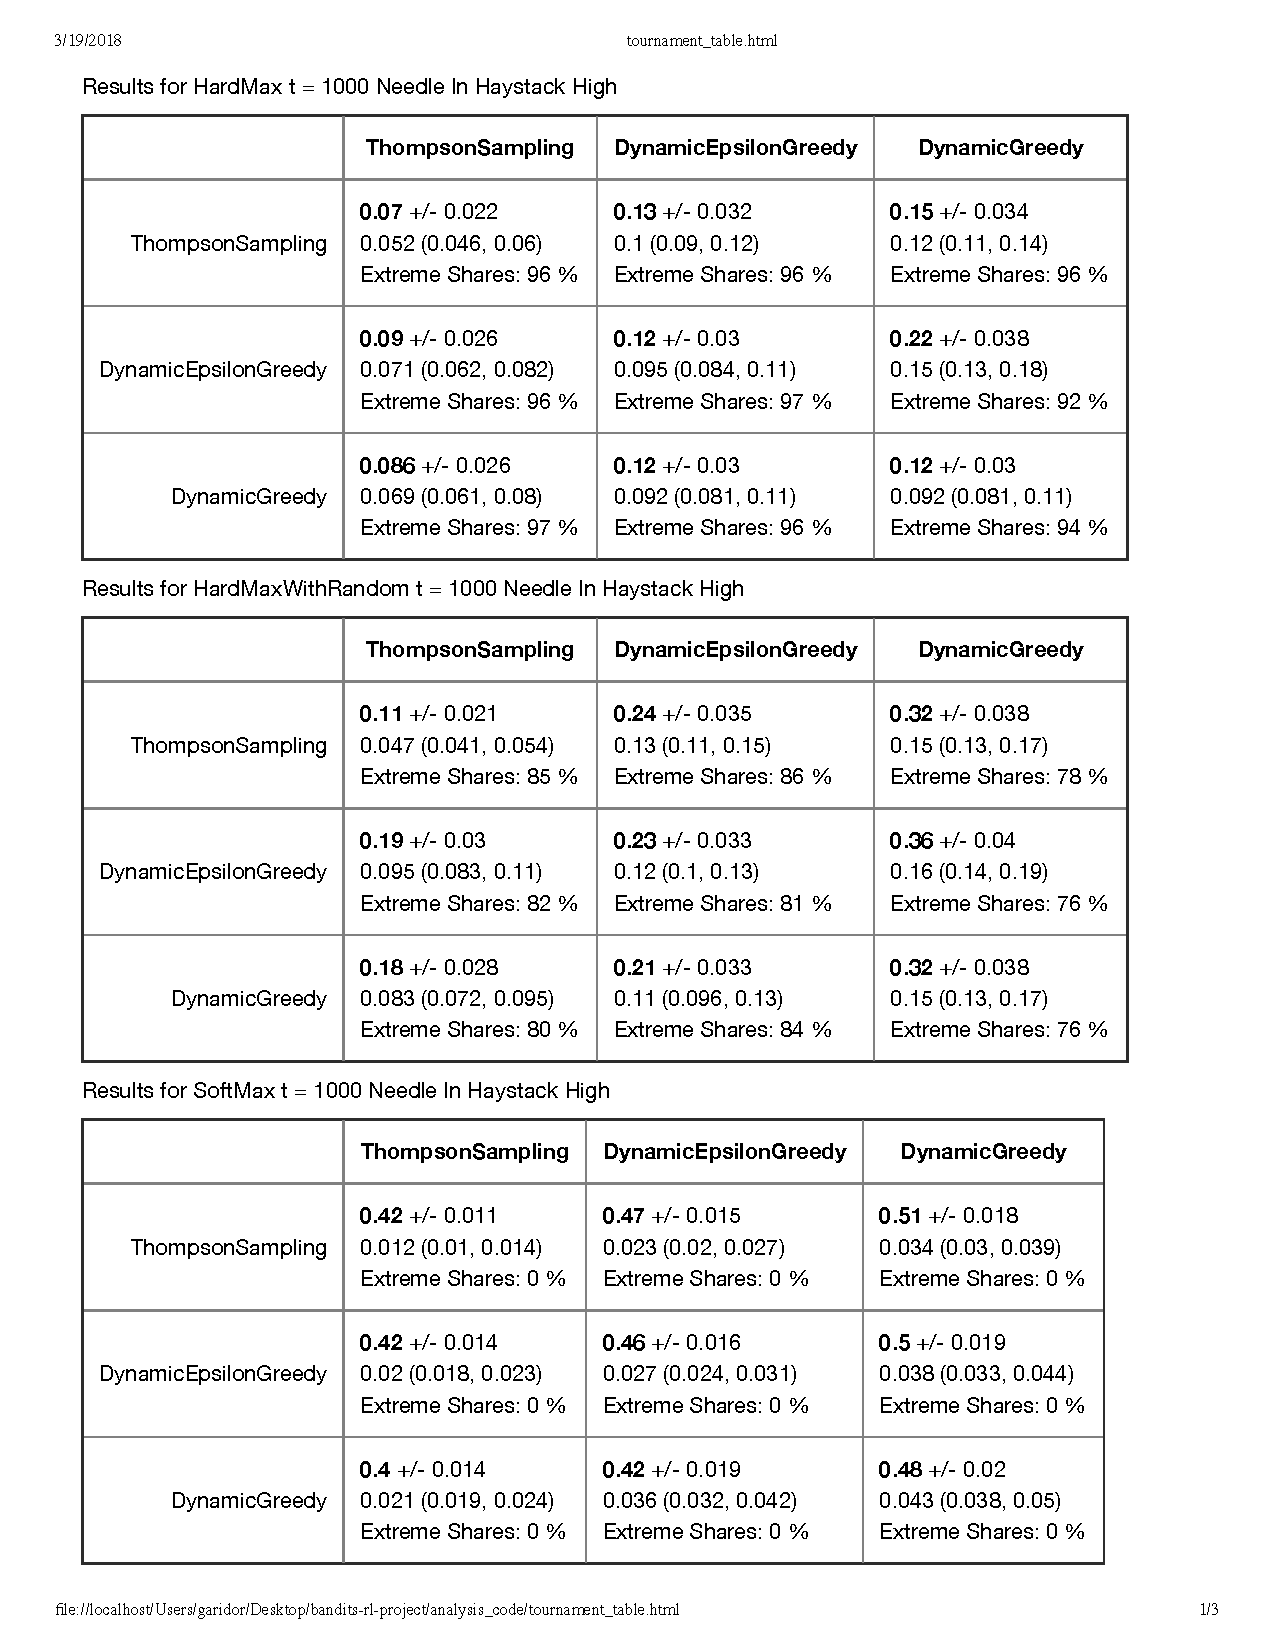
\includepdf[pages={-}]{more_memory_tournament_table}





\end{document}